\documentclass[11pt,xcolor=table]{beamer}

\usetheme[progressbar=frametitle]{metropolis}
\usepackage{appendixnumberbeamer}
\usepackage{pgfpages}
%\setbeameroption{show notes on second screen}
  \setbeamertemplate{enumerate items}[square]
\usepackage{multirow}

\usepackage{graphicx}

\usepackage{xcolor}

\newcommand{\link}[3][mLightBrown]{\href{#2}{\color{#1}{#3}}}%


\newcommand{\questionslide}[0]{
{\setbeamercolor{palette primary}{fg=black, bg=yellow}
\begin{frame}[standout]
    \raggedright
  Any questions? \\ \vspace{1cm}
  \raggedleft
  \dots{ } Remember -- Every question is useful!
\end{frame}
}}

\newcommand{\task}[1]{
   \begin{alertblock}
   {\centering \vspace{-1.5ex} \\ #1  \\ \vspace{-1.5ex} }
   \end{alertblock}
   }

\setbeamercolor{block title alerted}{%
    use={block title, alerted text},
    bg=yellow,
    fg=black
}

\definecolor{peppermint}{RGB}{75, 161, 115}
%\definecolor{peppermint}{RGB}{75, 161, 115}


\setbeamercolor{alerted text}{fg=peppermint , bg= black}

\usepackage{booktabs}
\usepackage[scale=2]{ccicons}

\usepackage{pgfplots}
\usepgfplotslibrary{dateplot}

\makeatletter 
\def\beamer@framenotesbegin{% at beginning of slide
    \usebeamercolor[fg]{normal text}
    \gdef\beamer@noteitems{}% 
    \gdef\beamer@notes{}% 
}
\makeatother


\usepackage{xspace}
\newcommand{\themename}{\textbf{\textsc{metropolis}}\xspace}

\title{Instrumental Variables: Practice
}
\subtitle{Econ 140, Section 8}
% \date{\today}
\date{}
\author{Jonathan Old}

% \titlegraphic{\hfill\includegraphics[height=1.5cm]{logo.pdf}}

\begin{document}

\maketitle

\begin{frame}{Roadmap}
  \setbeamertemplate{section in toc}[sections numbered]
  \tableofcontents%[hideallsubsections]
\end{frame}




\questionslide



\section{(Group) data projects}



\begin{frame}{Your time for questions}
I prepared a document that can help you find data if you are lost. See it \link{https://docs.google.com/document/d/1jk2HeniO9-yWuK9wG_iPcWnWQooZdlzhRWYWYSSqG4Q/edit?usp=sharing}{here}.

Let's take some time and go over your topics and strategies.

\end{frame}




\section{Introduction to Instrumental Variables}

\begin{frame}{Recap: Omitted Variable Bias}
    \begin{figure}
        \centering
        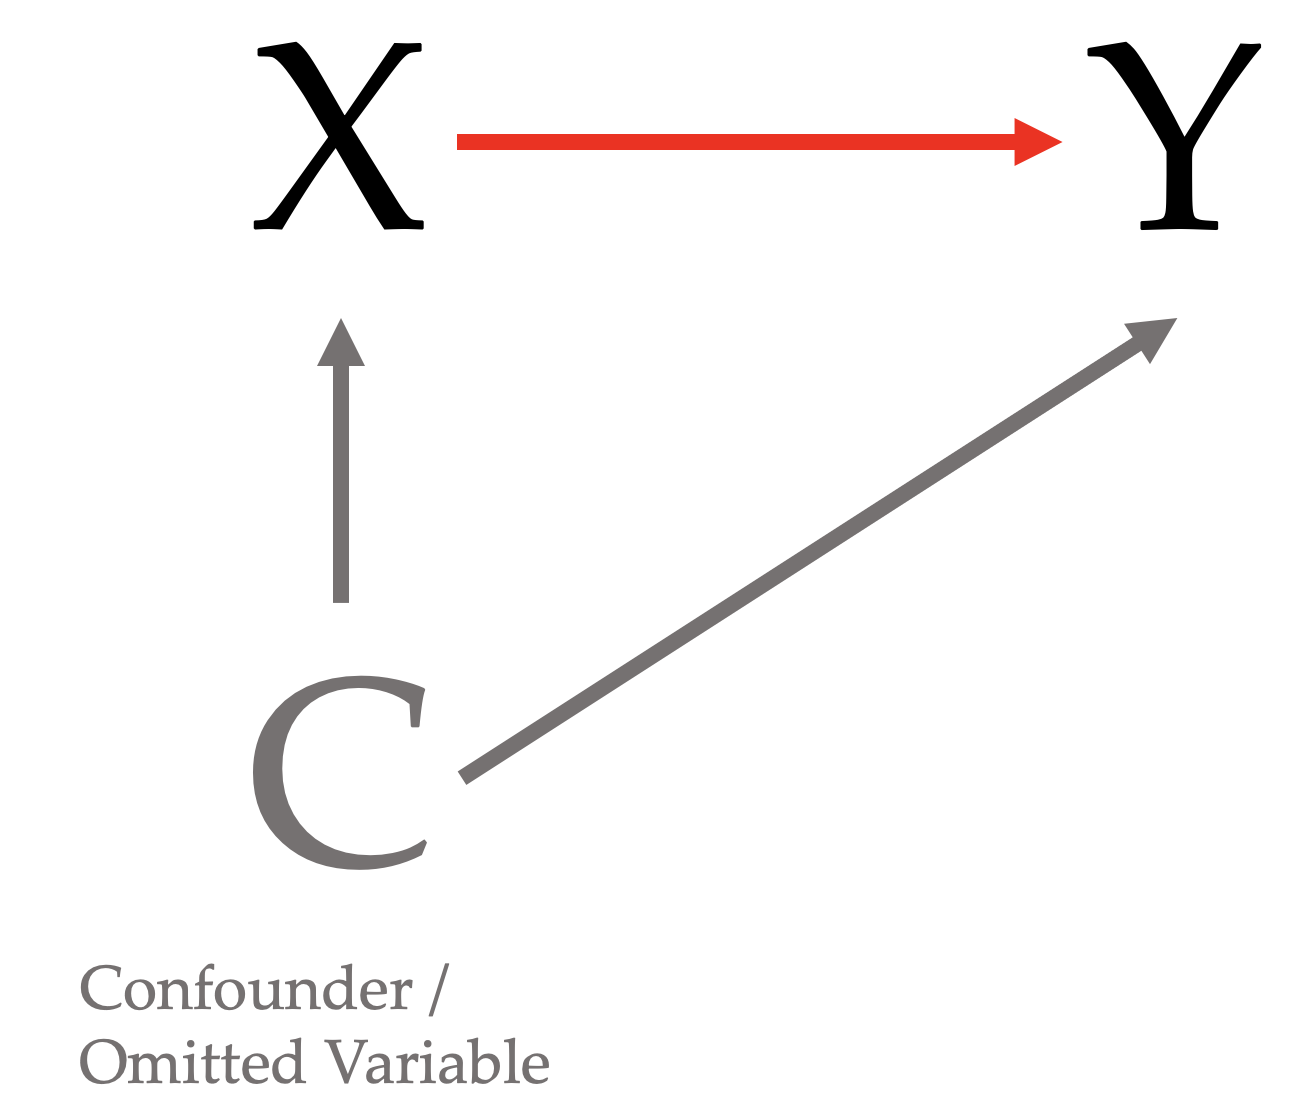
\includegraphics[width=0.5\textwidth]{DAGs/ovb.png}
       % \caption{IV setup}
        \label{fig:ovb}
    \end{figure}
\end{frame}



\begin{frame}{Instrumental variables: The setup}
    \begin{figure}
        \centering
        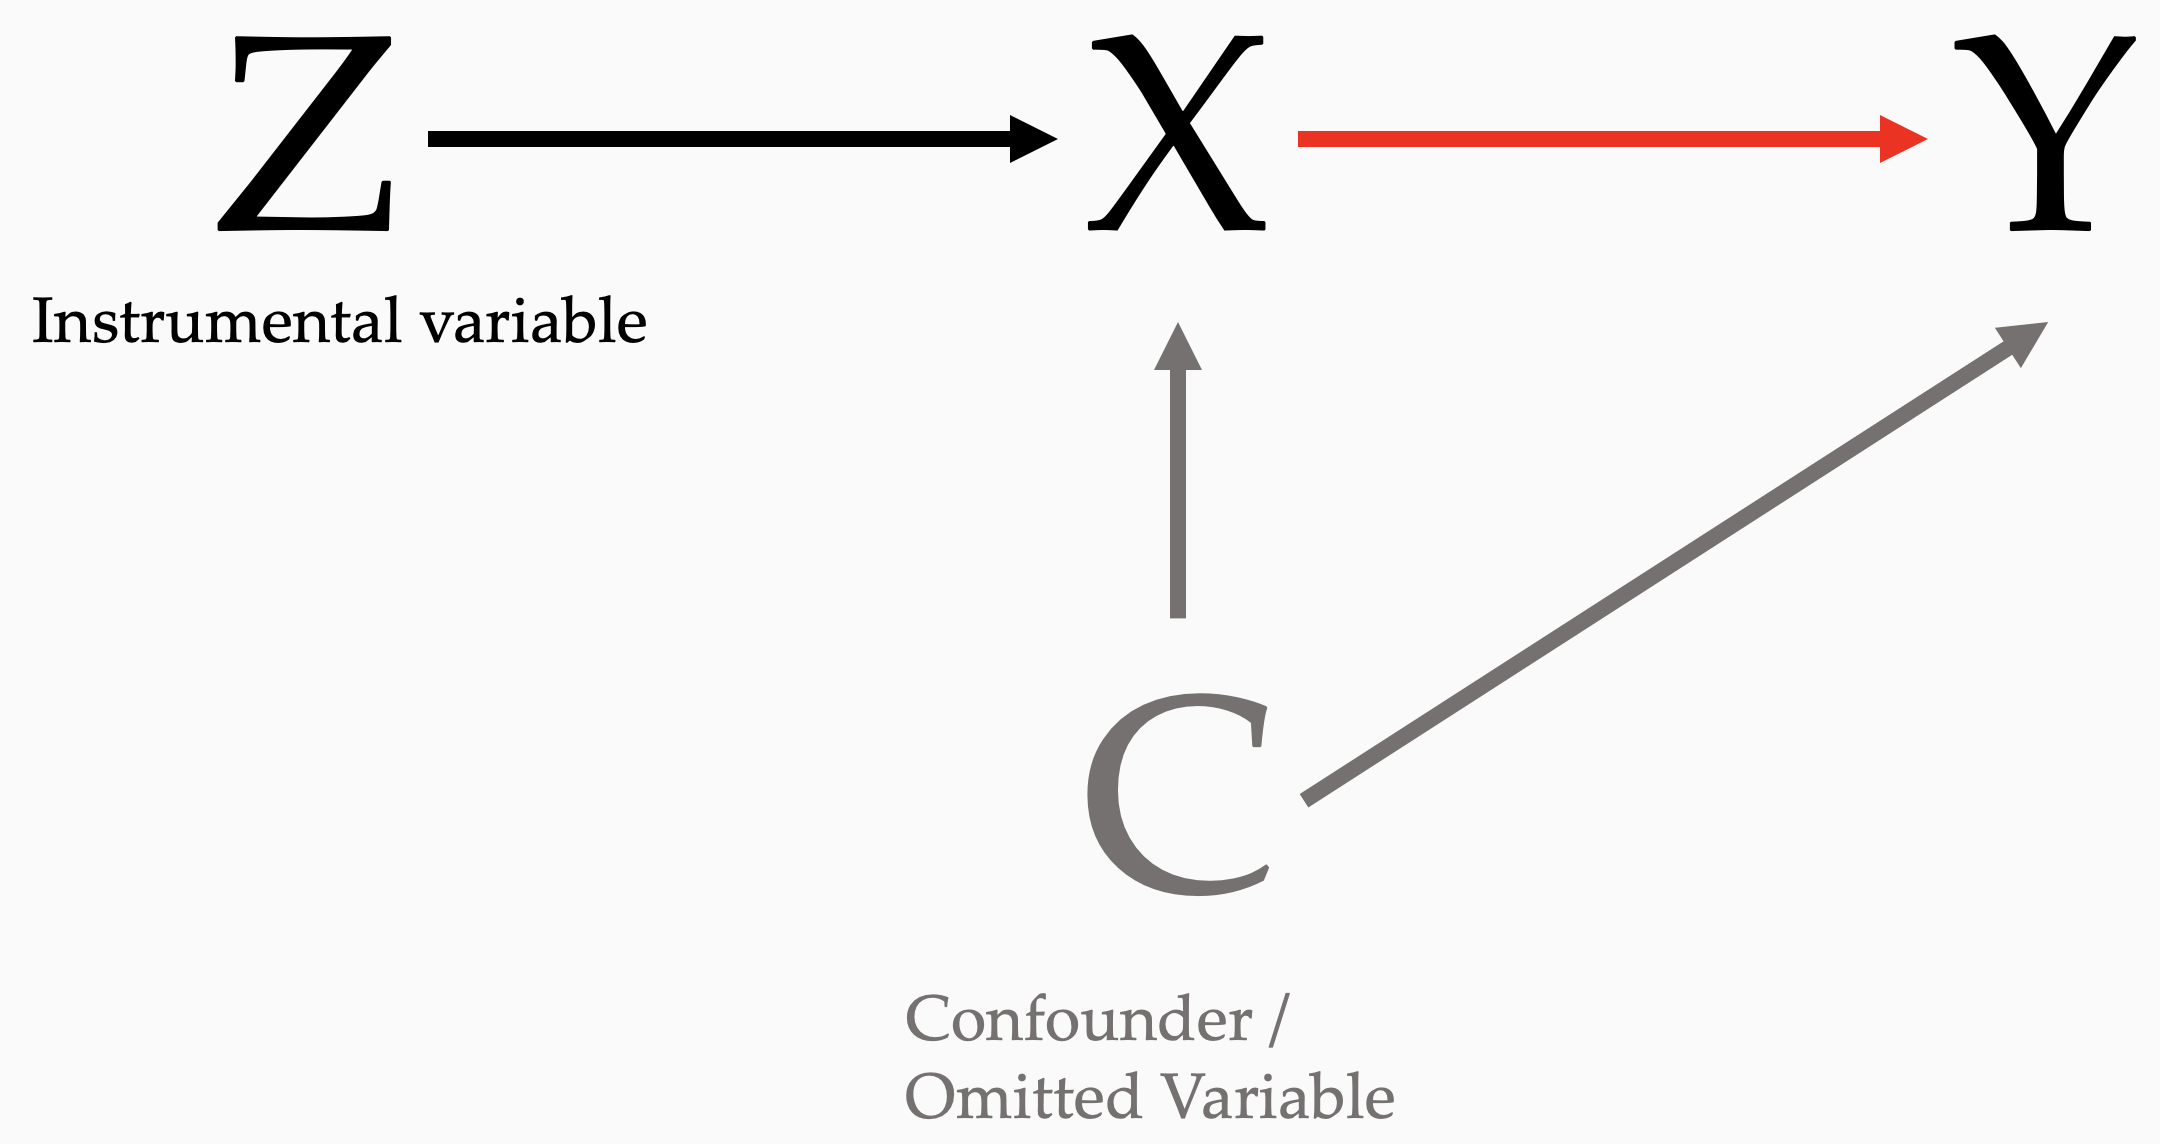
\includegraphics[width=0.8\textwidth]{DAGs/iv_simple.png}
       % \caption{IV setup}
        \label{fig:iv}
    \end{figure}
\end{frame}



\begin{frame}{Recap: IV "rescales" the effect}
    \begin{figure}
        \centering
        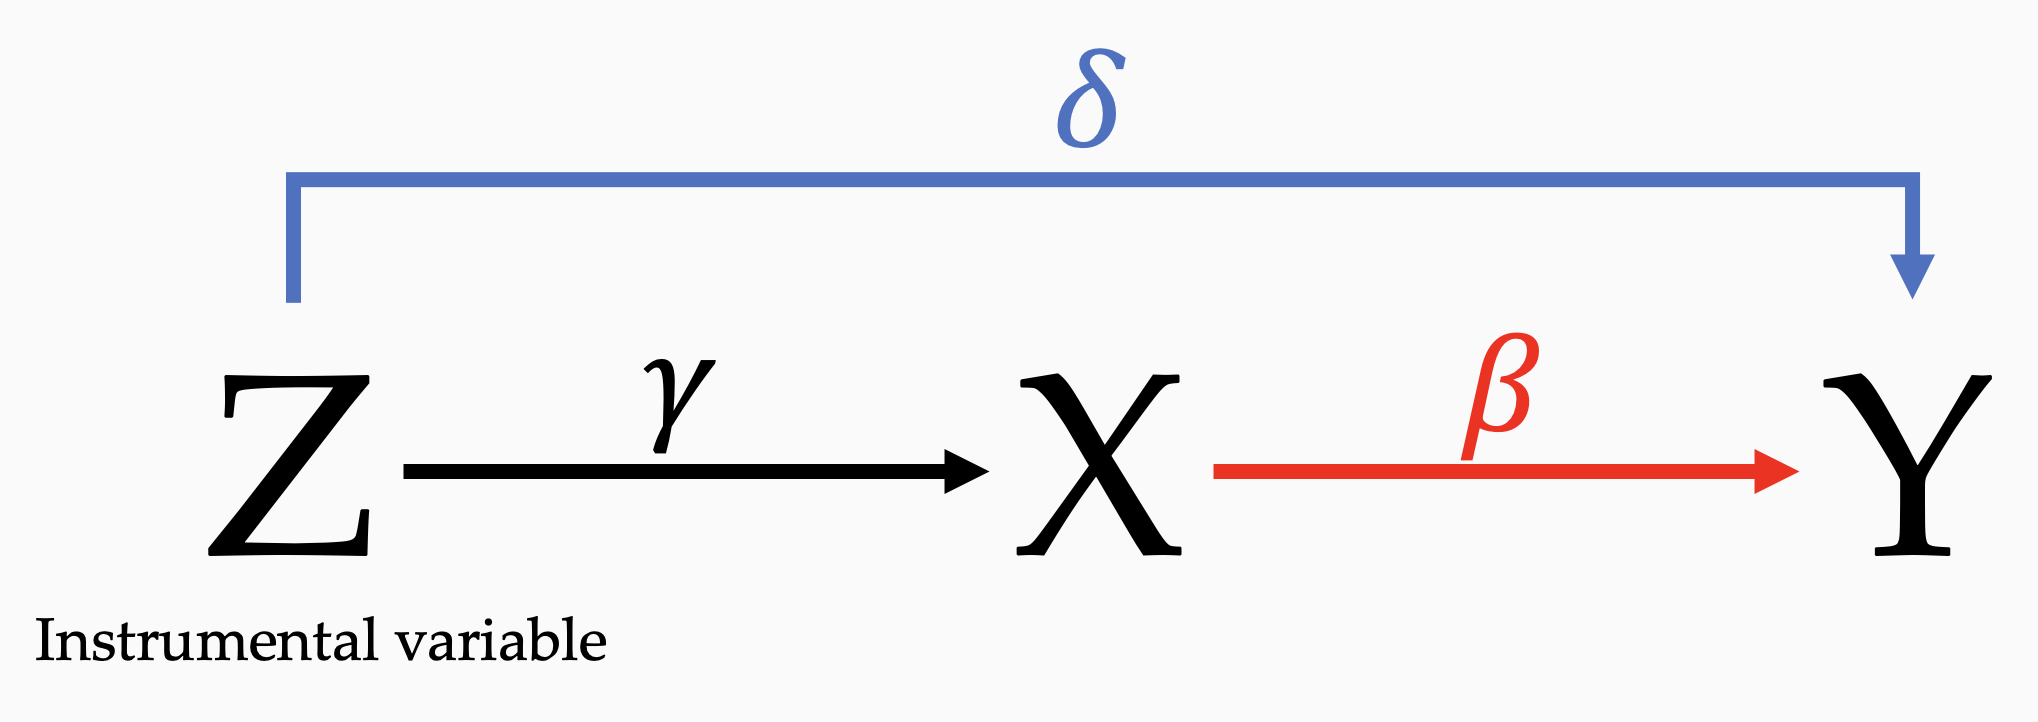
\includegraphics[width=0.75\textwidth]{DAGs/iv_calc.png}
       % \caption{We can calculate $\beta$ as $\delta / \gamma $.}
        \label{fig:iv2}
    \end{figure}
    
    A simple example: 
    \begin{itemize}
    \item We want to know the effect of chocolate ($X$) on happiness ($Y$), using a randomized voucher as instrument ($Z$). 
    \item We find: people with voucher were 3 points more happy ($\delta = 3$), and ate  0.5 more chocolates ($\gamma=0.5$).
    \item Then, the effect of eating one more chocolate is: \pause  $\beta = \delta / \gamma = 3/0.5= 6$.
    \end{itemize}
\end{frame}







\begin{frame}{IV in R}


\alert{Let's see how IV and 2SLS works on \texttt{\alert{\href{https://datahub.berkeley.edu/hub/user-redirect/git-pull?repo=https\%3A\%2F\%2Fgithub.com\%2Fryanedw\%2FECON-140-FA23-RDE&branch=main&urlpath=tree\%2FECON-140-FA23-RDE\%2F}{Datahub}}}}
\end{frame}







\begin{frame}{Calculating the IV coefficient}
    
What is the effect of \textbf{eating chocolate} (D) on happiness (Y).
\begin{itemize}
    \item Why not estimate: $Y_i = \alpha + \beta D_i + \varepsilon_i$?
\end{itemize}
\textbf{Randomly} give voucher to buy chocolate at $90 \%$ discount (Z).

\begin{itemize}
    \item Why not estimate: $Y_i = \alpha + \beta Z_i + \varepsilon_i$?
\end{itemize}
\textbf{Let us set up some regressions}:
\begin{align*}
\text{Regression of interest: }  Y_i&=\alpha+\beta  D_i +  e_i \\
\text{First stage: }  D_i&=\alpha_1+\gamma  Z_i + u_i \\
\text{Reduced Form: }  Y_i&=\alpha_2+\delta  Z_i + v_i \\
\text{Plug in regression of interest: }  Y_i &= \alpha + \beta (\alpha_1+\gamma \cdot Z_i + u_i) + e_i   \\ 
\text{Get back reduced form: \qquad }& = \underbrace{(\alpha + \beta \alpha_1)}_{\alpha_2} + \underbrace{(\beta \gamma)}_{\delta} Z_i + \underbrace{(\beta u_i + e_i)}_{v_i}  \\
 \text{So we see that} \qquad    \delta = \beta \gamma &\Leftrightarrow \beta = \delta / \gamma
\end{align*}





\end{frame}






\begin{frame}{IV gives us the treatment effect for the compliers}

\begin{figure}
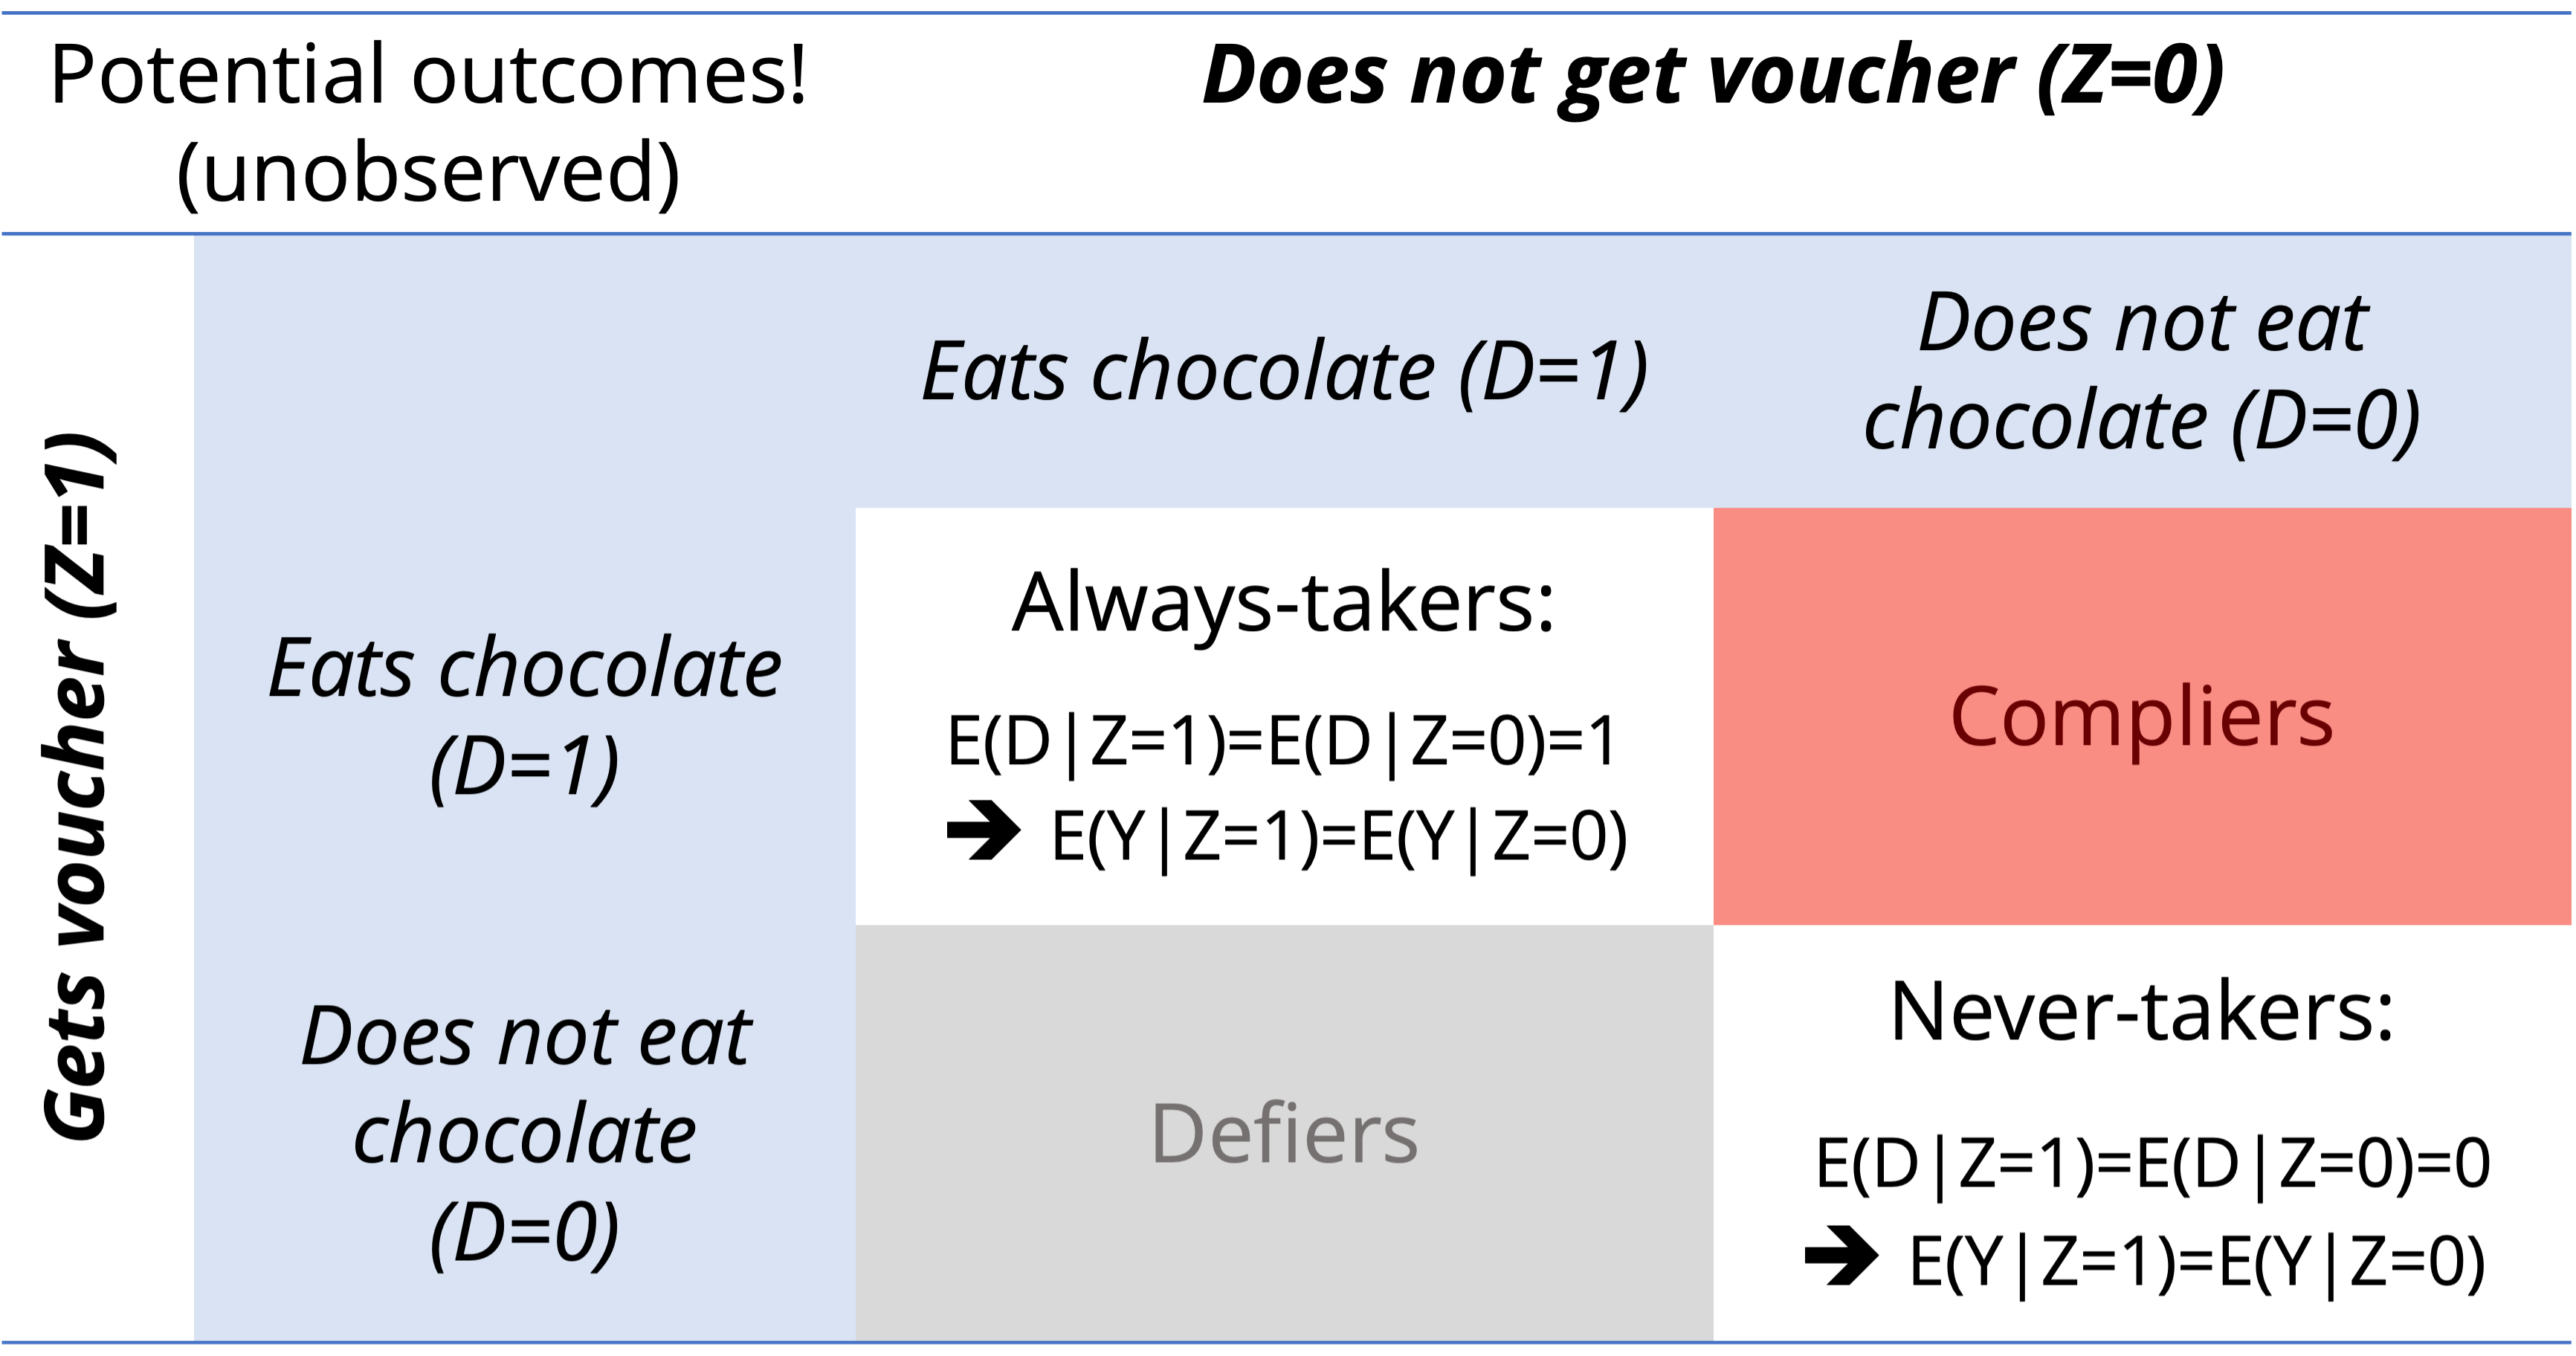
\includegraphics[width=\textwidth]{figures/iv_table.png}
\end{figure}

\end{frame}





\section{IV Summary}



\begin{frame}{IV summary}

We need the following three assumptions for IV to work: 
    \begin{enumerate}
    \item \textbf{Relevance}: $Z$ must truly affect $X$
    \item \textbf{Independence/Exogeneity}: $Z$ is as good as randomly assigned
    \item \textbf{Exclusion Restriction}: The \textbf{only} way that $Z$ affects $Y$ is via $X$.
    \end{enumerate}



    \begin{figure}
 
        \centering
        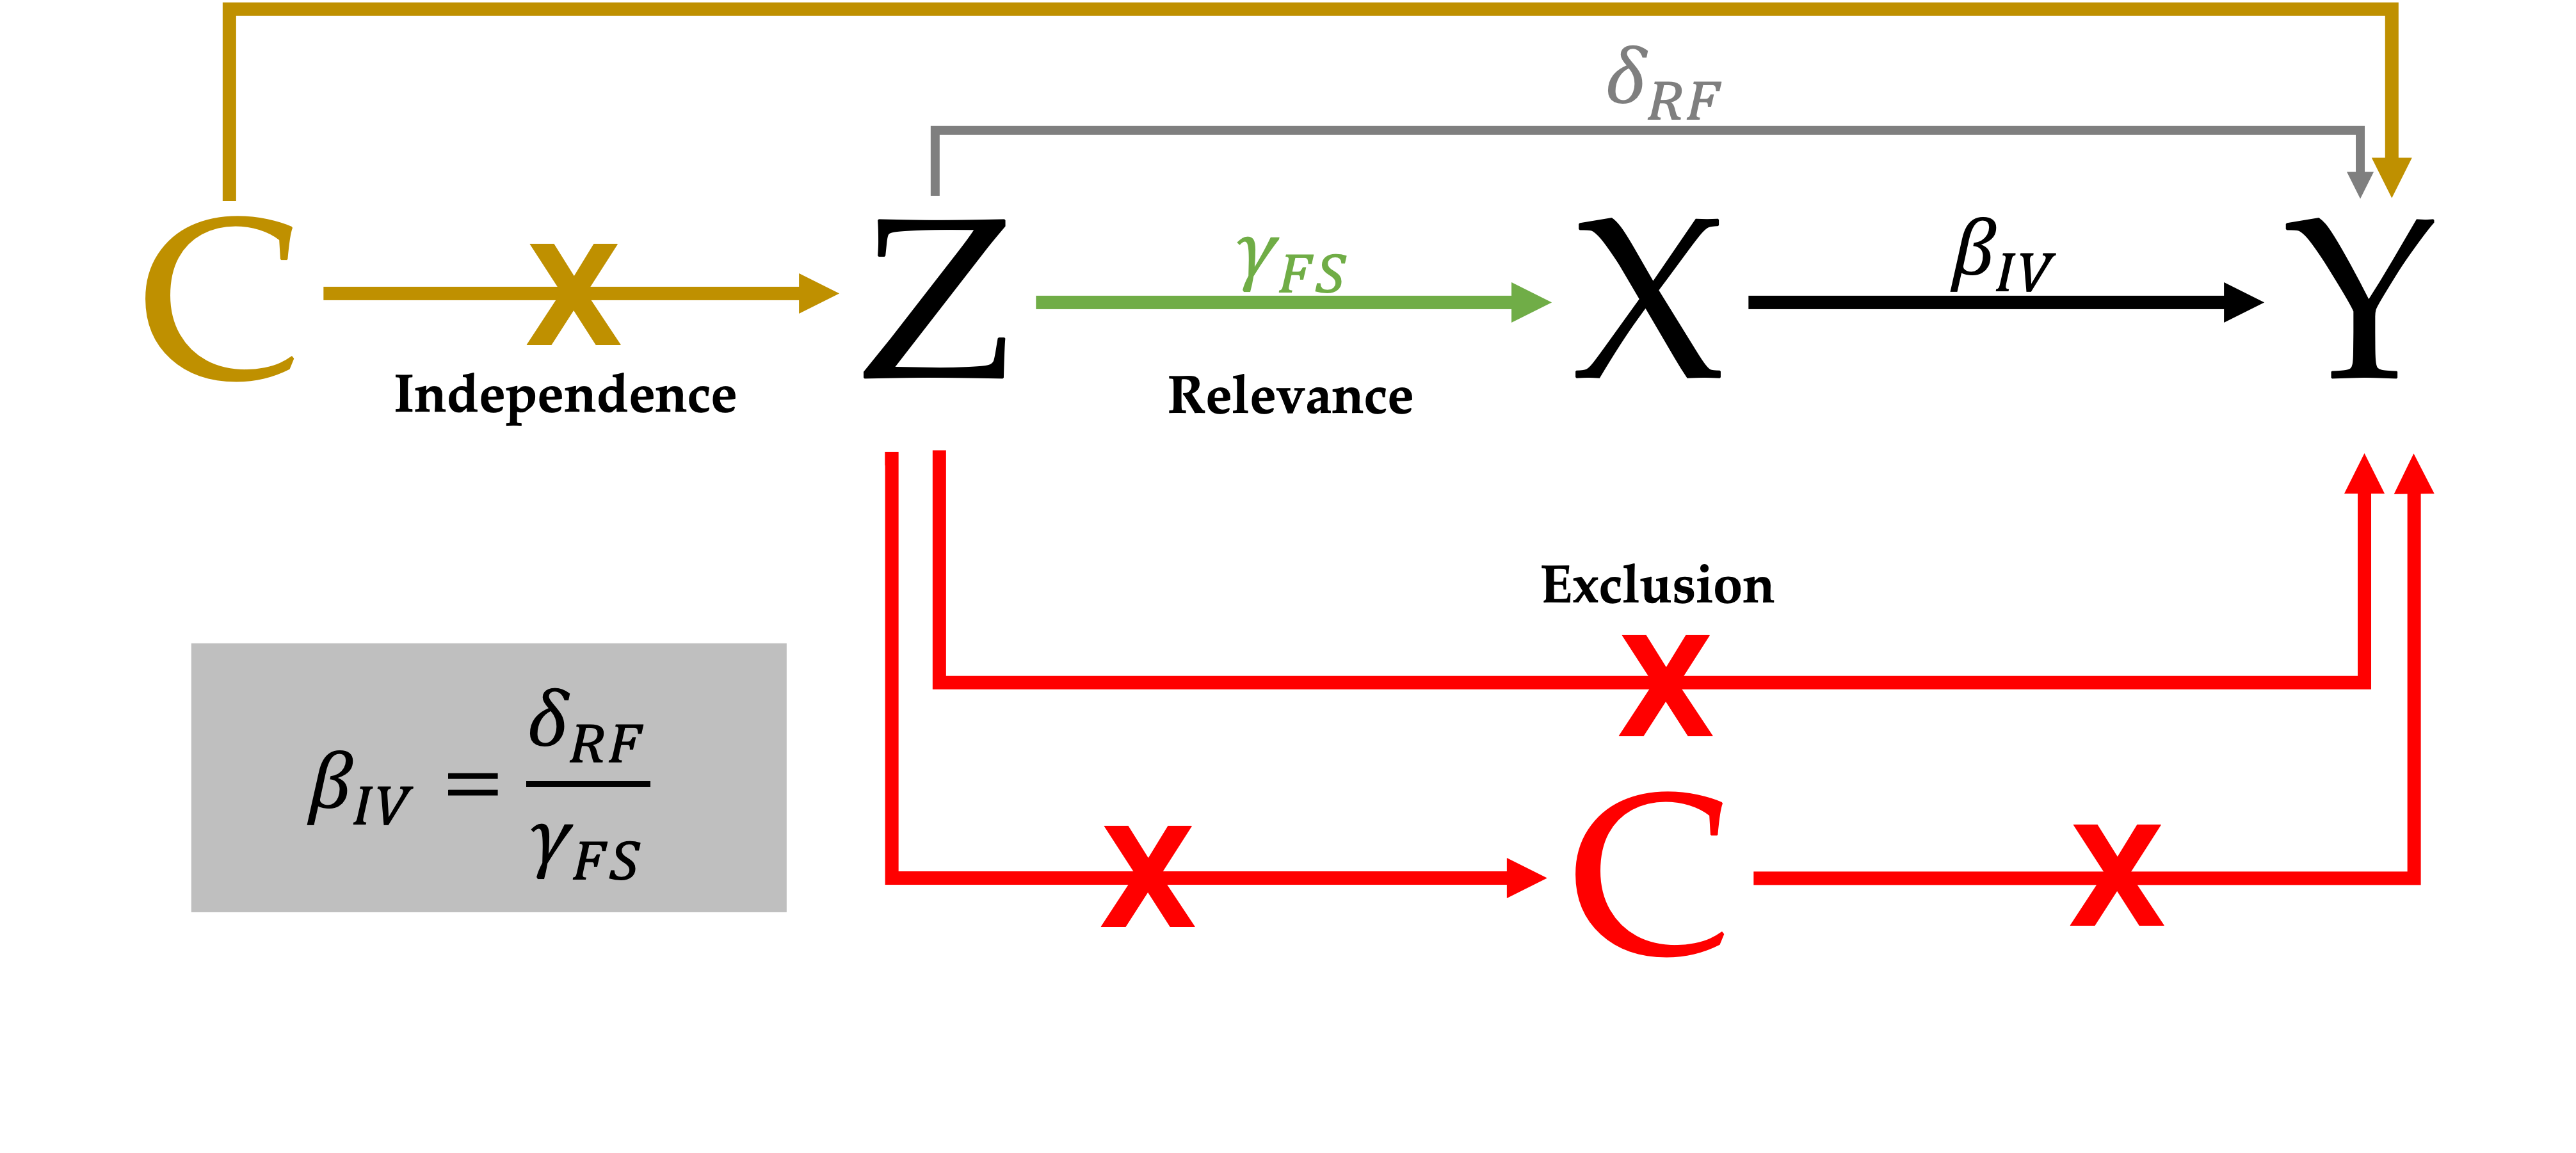
\includegraphics[width=1\textwidth]{DAGs/iv_summary_full.png}
        %\caption{Almost all you need to know about IVs!}
        \label{fig:iv3}
    \end{figure}
    
   \end{frame}


















\questionslide


\section{Rainfall IV}

\begin{frame}{Intro}

\includegraphics[width=\textwidth]{figures/IV Rain/iv_intro.png}

\end{frame}



\begin{frame}{Why IV?}
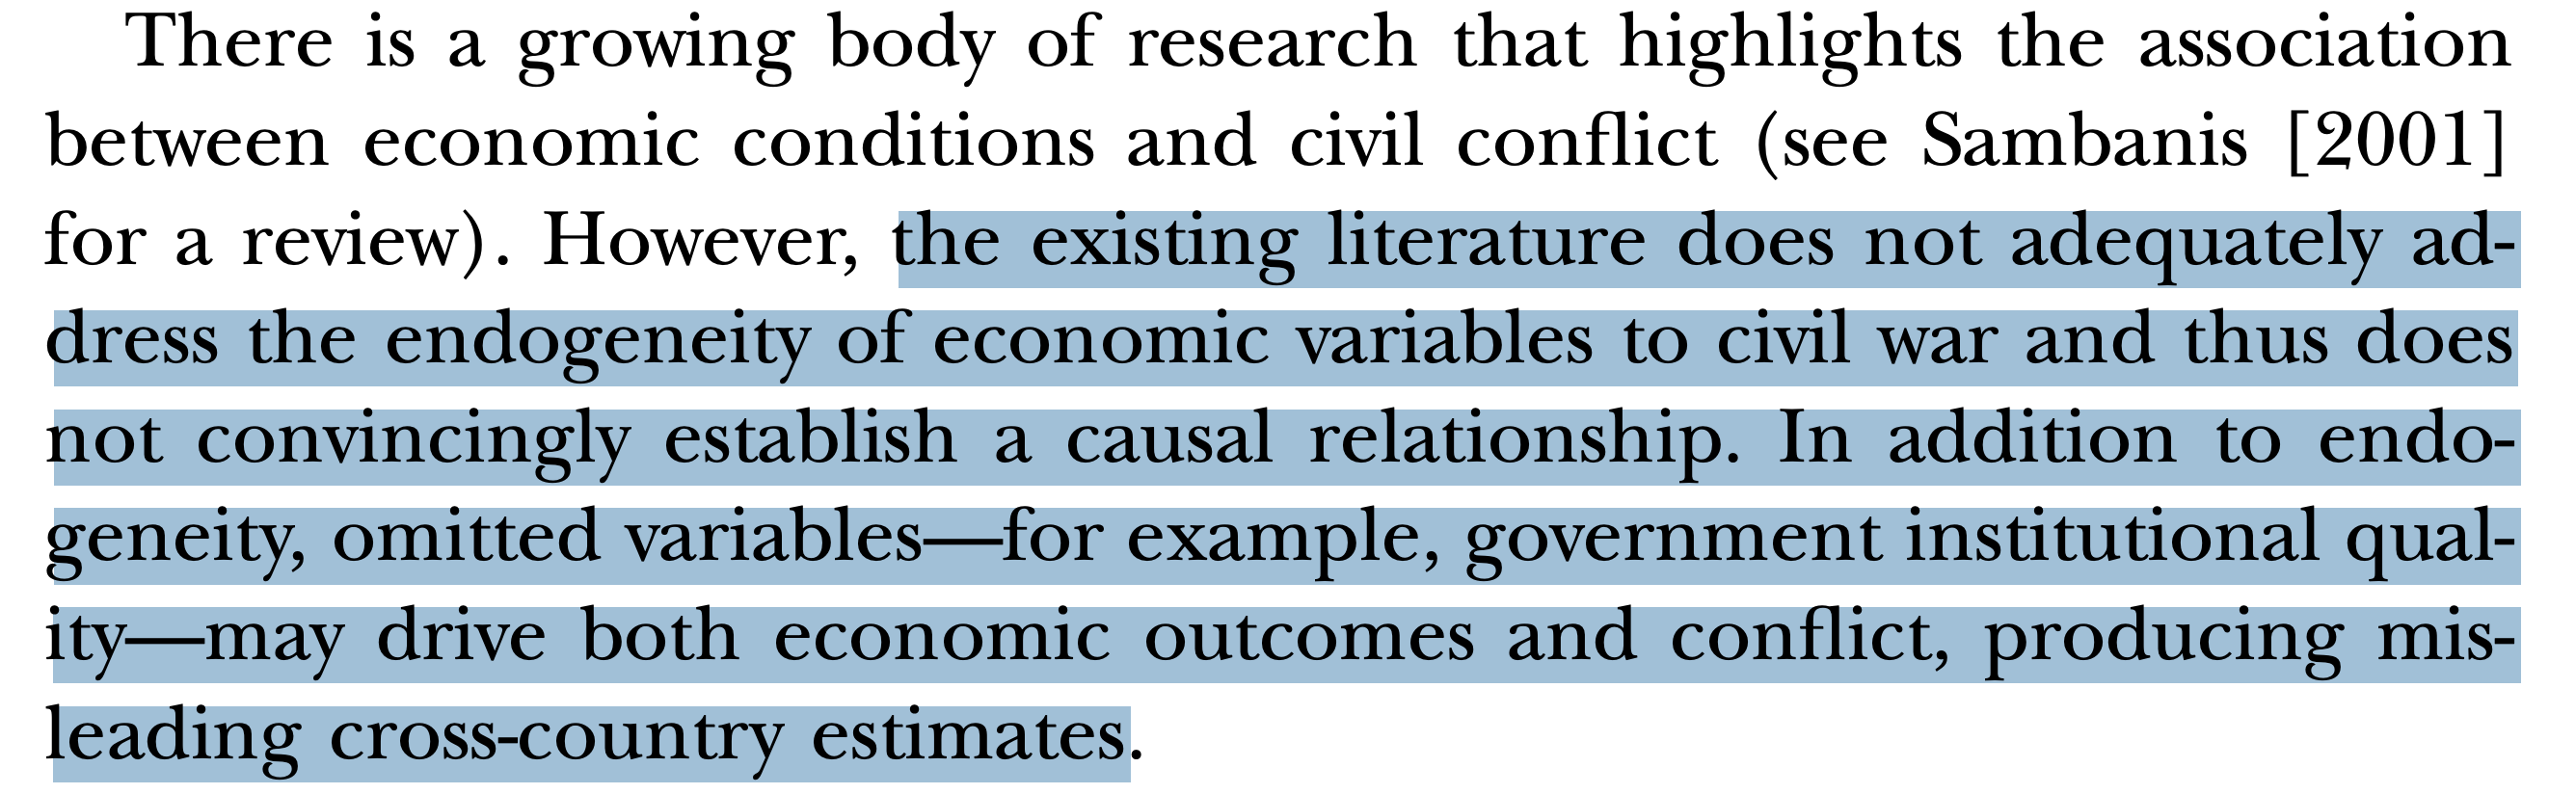
\includegraphics[width=\textwidth]{figures/IV Rain/whyiv.png}
\end{frame}


\begin{frame}{Relevance}

\includegraphics[width=\textwidth]{figures/IV Rain/relevance.png}
\end{frame}


\begin{frame}{Exclusion}
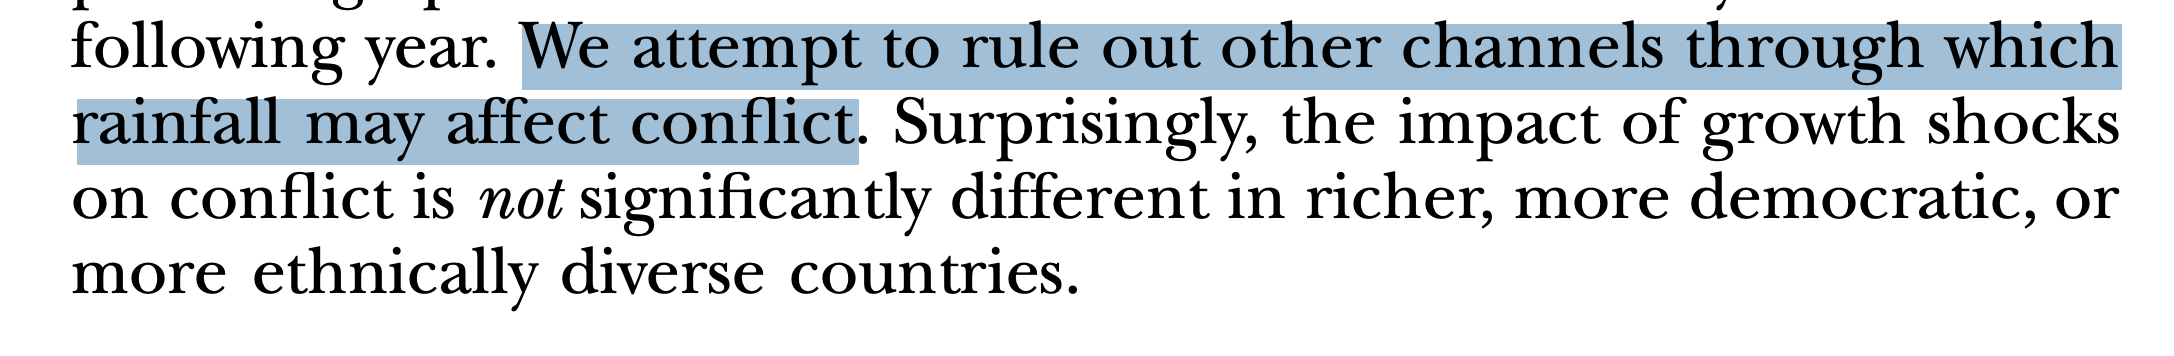
\includegraphics[width=\textwidth]{figures/IV Rain/exclusion.png}
\end{frame}



\begin{frame}{Exclusion}

\includegraphics[width=\textwidth]{figures/IV Rain/exclusion 1.png}
\end{frame}


\begin{frame}{Exclusion}
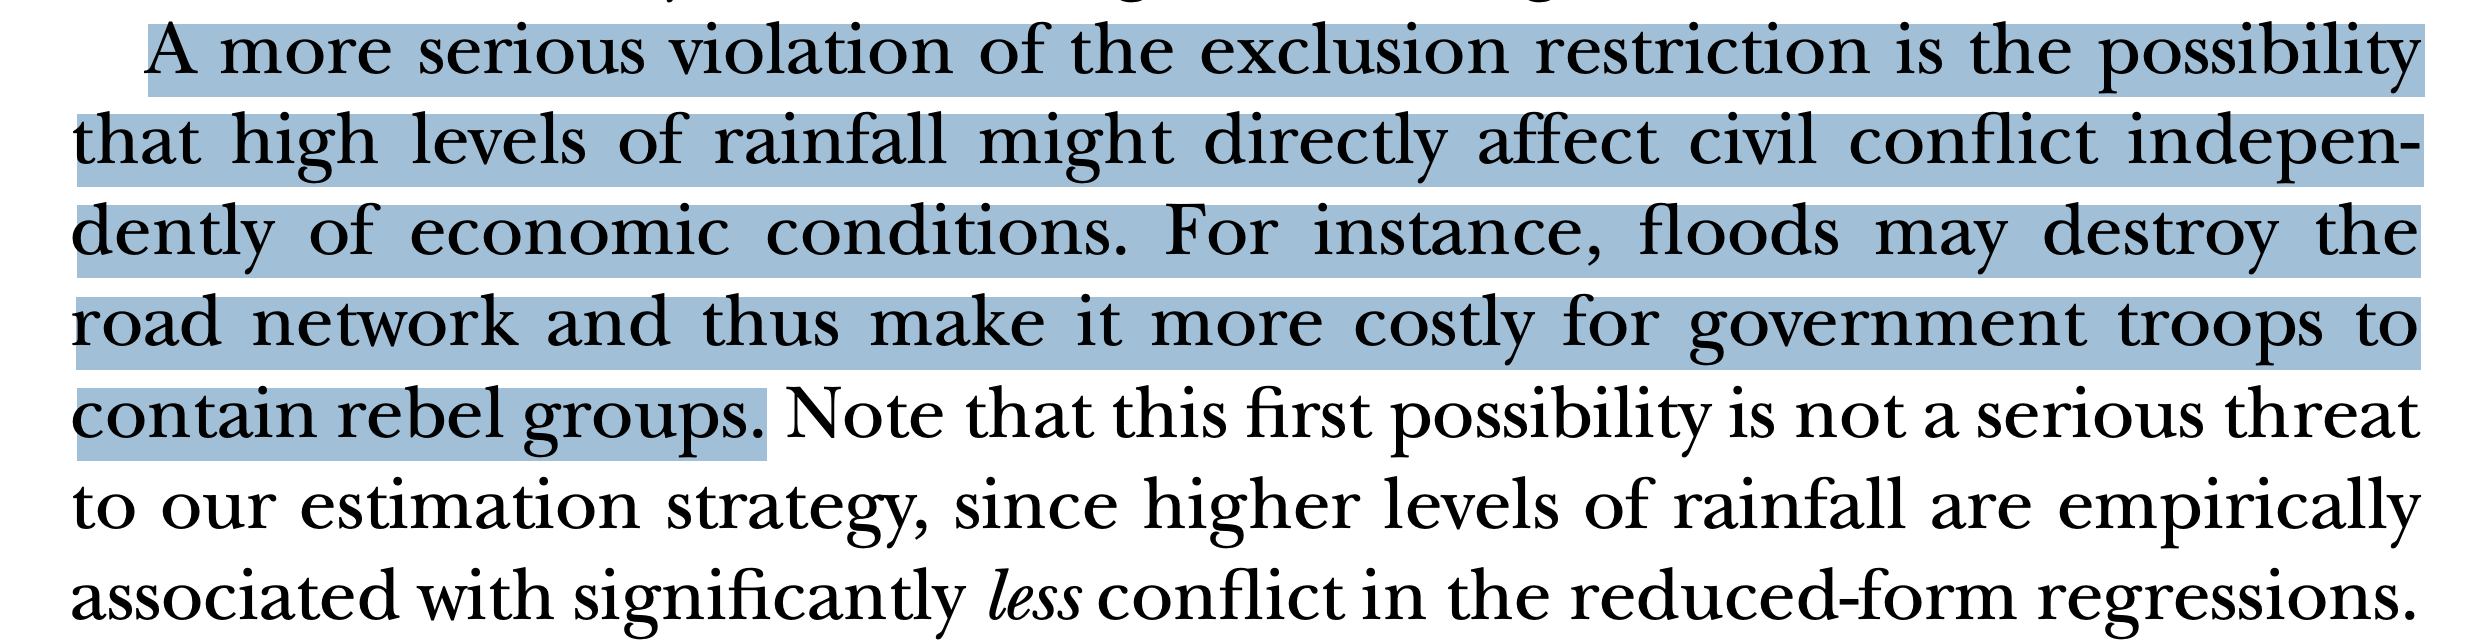
\includegraphics[width=\textwidth]{figures/IV Rain/exclusion 2.png}
\end{frame}


\begin{frame}{Exclusion}
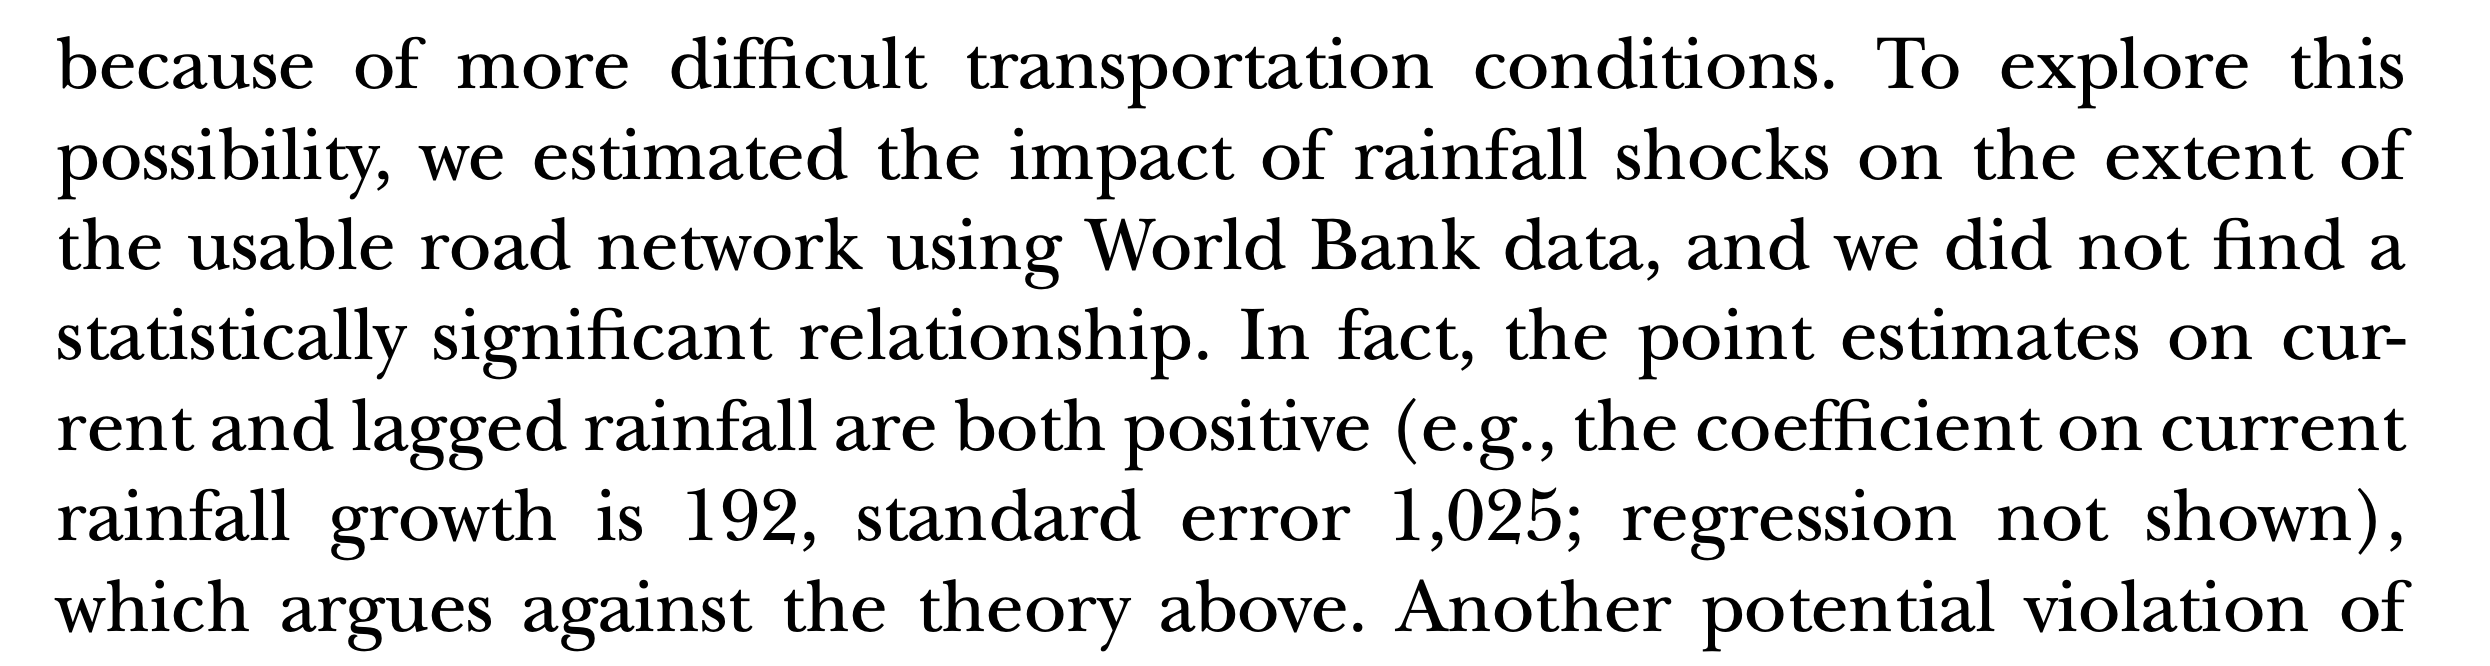
\includegraphics[width=\textwidth]{figures/IV Rain/exclusion 3.png}
\end{frame}




\begin{frame}{Interested in these topics?}

\href{https://freakonomics.com/podcast/edward-miguel-on-collecting-economic-data-by-canoe-and-correlating-conflict-with-rainfall/}{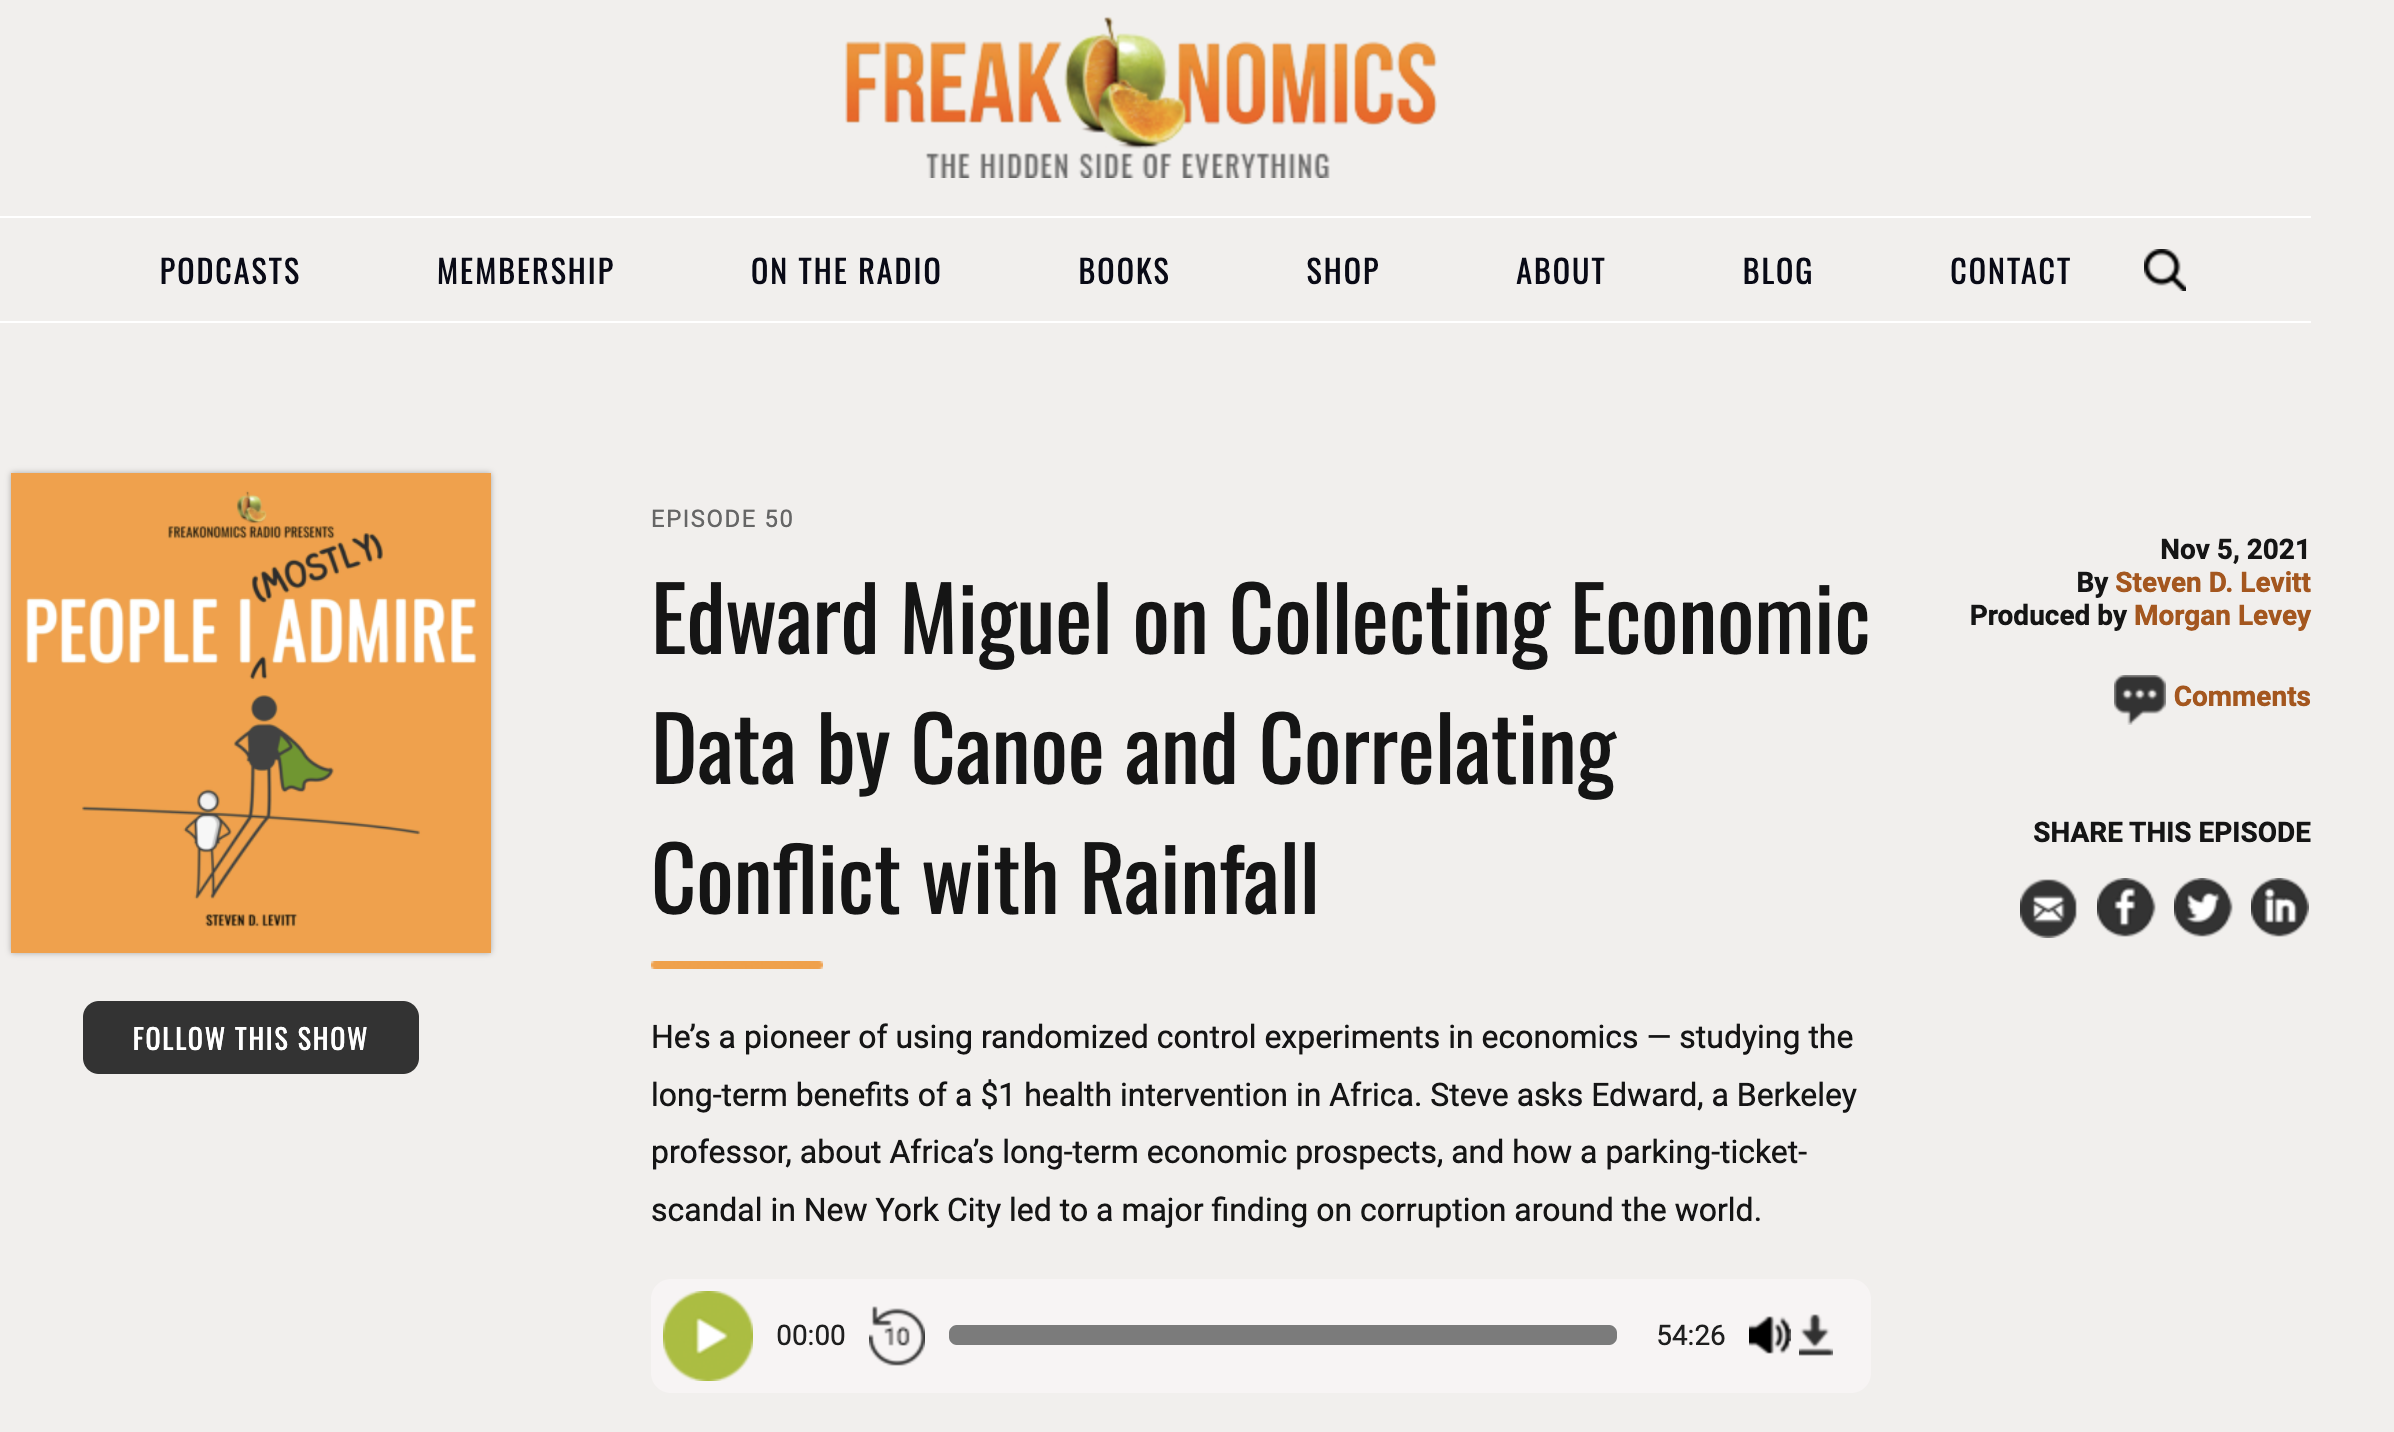
\includegraphics[width=\textwidth]{figures/IV Rain/freakonomics.png}}

\end{frame}


\section{Group work}



\begin{frame}{Group work}

    \begin{itemize}
    
    
\item[\textit{Group 1:}] We are interested in the effect of being in the army on crime. We instrument being in the army with a lottery (\link{https://www.aeaweb.org/articles?id=10.1257/app.3.2.119}{paper})

\item[\textit{Group 2:}]  We are interested in the effect of protestant religion on economic growth. We instrument protestantism in a region with the distance to Wittenberg (\link{https://academic.oup.com/qje/article/124/2/531/1905076}{paper})

%\item[\textit{Group 2:}]  We are interested in the effect of income on conflict. We instrument income with rainfall (\link{https://www-journals-uchicago-edu.libproxy.berkeley.edu/doi/10.1086/421174}{paper})


\item[\textit{Group 3:}]  We are interested in the effect of air pollution on mortality. We instrument local air pollution with wind direction (\link{https://www.aeaweb.org/articles?id=10.1257/aer.20180279}{paper})



       \end{itemize}

\begin{enumerate}
	\item Relevance: Z must truly affect X
	\item Independence/Exogeneity: Z is as good as randomly assigned
	\item Exclusion restriction: The \textbf{only} way that Z affects Y is via X
\end{enumerate}

%\textbf{\alert{Your job: Discuss whether these three assumptions hold!!}}

 %  \begin{alertblock} {\centering \vspace{-1.5ex} \\ Your job: Discuss whether these three assumptions hold!  \\ \vspace{-1.5ex} } \end{alertblock}
    
    \task{Your job: Discuss whether these assumptions hold!}
   \end{frame}







\questionslide




\end{document}
